\documentclass{article}
\pdfpagewidth=8.5in
\pdfpageheight=11in

\usepackage{ijcai23}

\usepackage{times}
\usepackage{soul}
\usepackage{url}
\usepackage[hidelinks]{hyperref}
\usepackage[utf8]{inputenc}
\usepackage[small]{caption}
\usepackage{graphicx}
\usepackage{amsmath}
\usepackage{amsthm}
\usepackage{booktabs}
\usepackage[switch]{lineno}

\usepackage{listings}
\usepackage[linesnumbered,ruled,vlined]{algorithm2e}
\usepackage[capitalize,noabbrev]{cleveref}
\usepackage{microtype}
\usepackage{amsfonts}
\usepackage{mathtools}
\usepackage{tikz}

% Comment out this line in the camera-ready submission
\linenumbers

\urlstyle{same}

% the following package is optional:
%\usepackage{latexsym}

% See https://www.overleaf.com/learn/latex/theorems_and_proofs
% for a nice explanation of how to define new theorems, but keep
% in mind that the amsthm package is already included in this
% template and that you must *not* alter the styling.
\newtheorem{example}{Example}
\newtheorem{theorem}{Theorem}
\newtheorem{definition}{Definition}
\newtheorem*{remark}{Remark}
\newtheorem{fact}{Fact}

% PDF Info Is REQUIRED.
% Please **do not** include Title and Author information
\pdfinfo{
/TemplateVersion (IJCAI.2023.0)
}

\lstset{breaklines=true}
\lstset{language=C++,
        basicstyle=\ttfamily,
        stringstyle=\color{red},
        commentstyle=\color{green},
        breaklines=true,
        showstringspaces=false}

\crefname{line}{line}{lines}
\crefalias{formula}{equation}
\crefname{formula}{Clause}{Clauses}
\creflabelformat{formula}{#2\textup{(#1)}#3}

\DeclareMathOperator{\Dom}{Dom}
\DeclareMathOperator{\Doms}{Doms}
\DeclareMathOperator{\Preds}{Preds}
\DeclareMathOperator{\Vars}{Vars}
\DeclareMathOperator*{\argmin}{argmin}
\newcommand{\expr}{\mathtt{expr}}

\SetKwFunction{Crane}{Crane}
\SetKwFunction{Propagate}{Propagate}
\SetKwFunction{FindBaseCases}{FindBaseCases}

\usetikzlibrary{arrows.meta}
\usetikzlibrary{positioning}
\usetikzlibrary{shapes}
\usetikzlibrary{fit}

\title{Towards Practical First-Order Model Counting}

% \author{
% First Author$^1$
% \and
% Second Author$^2$\and
% Third Author$^{2,3}$\And
% Fourth Author$^4$
% \affiliations
% $^1$First Affiliation\\
% $^2$Second Affiliation\\
% $^3$Third Affiliation\\
% $^4$Fourth Affiliation
% \emails
% \{first, second\}@example.com,
% third@other.example.com,
% fourth@example.com
% }

\begin{document}

\maketitle

% <= 200 words
\begin{abstract}
\end{abstract}

\section{Introduction}

\begin{figure*}[t]
  \centering
  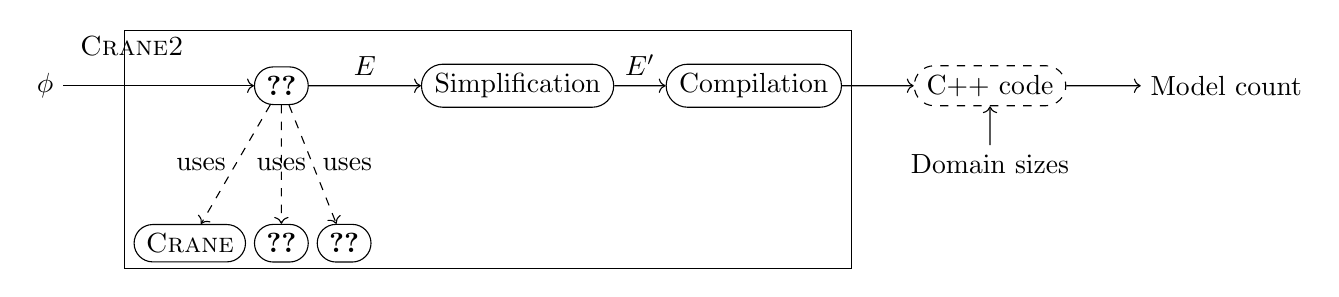
\begin{tikzpicture}
    \node at (0, 0) (formula) {$\phi$};
    \node[draw,rounded rectangle] at (3, 0) (alg1) {\Cref{alg:main}};
    \node[draw,rounded rectangle] at (6, 0) (simplification) {Simplification};
    \node[draw,rounded rectangle] at (9, 0) (compilation) {Compilation};

    \node[draw,rounded rectangle,dashed] at (12, 0) (cpp) {C++ code};
    \node at (12, -1) (sizes) {Domain sizes};

    \node at (15, 0) (count) {Model count};

    \node[draw,rounded rectangle] at (3, -2) (alg2) {\Cref{alg1}};
    \node[draw,rounded rectangle,left = 0.1cm of alg2] (crane) {\textsc{Crane}};
    \node[draw,rounded rectangle,right = 0.1cm of alg2] (alg3) {\Cref{alg2}};

    \node[draw,fit={(alg1) (simplification) (compilation) (crane) (alg2) (alg3)},inner ysep=7pt,yshift=5pt] {};
    \node at (1.1, 0.5) {\textsc{Crane2}};

    \draw[->] (formula) -- (alg1);
    \draw[->] (alg1) -- node[above] {$E$} (simplification);
    \draw[->] (simplification) -- node[above] {$E'$} (compilation);
    \draw[->] (compilation) -- (cpp);
    \draw[->] (sizes) -- (cpp);
    \draw[->] (cpp) -- (count);

    \draw[->,dashed] (alg1) -- node[midway,left] {uses} (crane);
    \draw[->,dashed] (alg1) -- node[midway] {uses} (alg2);
    \draw[->,dashed] (alg1) -- node[midway,right] {uses} (alg3);
  \end{tikzpicture}
  \caption{Using \textsc{Crane2} to compute the model count of formula $\phi$.\
    The formula is compiled into a set of equations $E$, which are then
    algebraically simplified and compiled to a C++ program. This program can
    then be run with different command line arguments to compute the model count
    of $\phi$ for various domain sizes.}
\end{figure*}

The evaluation of base cases is done by simplifying the clauses and then using
\textsc{Crane} to find the base cases. First, while traversing the graph to find
the equations, we store two maps: $\mathcal{F}$ (which stores the mapping from
the function names to the formulae, whose model count they represent) and
$\mathcal{D}$ (which stores the mapping from the variable names to the domains
whose sizes they represent). Then, a particular domain is selected (using the
algorithm described in previous reports), and the clauses are simplified. Then,
\textsc{Crane} is called on those clauses to evaluate the base cases. After
that, we change the function names and variable to make it consistent with the
previous domain to variable mapping, and append these base cases to the set of
equations.

\paragraph{Contributions.}
\begin{itemize}
  \item \Cref{sec:identifying}
  \item \Cref{sec:simplifying}
  \item Converting the recursive equations into a C++ program, which can then be
        compiled and executed to obtain numerical values (see \cref{sec:cpp}).
  \item Support for infinite precision integers using the GNU Multiple Precision
        Arithmetic Library.
  \item The experiments are (going to be) more comprehensive than any other
        experimental study performed on (W)FOMC algorithms (TODO: references to
        my previous paper and some of the \textsc{ForcLift} and
        \textsc{FastWFOMC} papers that contain experimental results).
\end{itemize}

\Cref{sec:identifying,sec:cpp} deal with algebraic constructs whereas
\cref{sec:simplifying} deals with logic.

\section{Preliminaries}

\subsection{Algebra}

\paragraph{Notation.}
We write $\expr{}$ for an arbitrary algebraic expression. For any signature or
clause $C$, argument or variable $x$, and number or constant $t$, we shall write
$C[t / x]$ for the result of substituting $t$ for all occurrences of $x$ in $C$.
% TODO: check if I'm still using this notation in all these cases
% TODO: explain how this works for function calls too

\begin{definition}
  A \emph{function call} is a term of the form
  $f(x_{1} - c_{1}, \dots, x_{n} - c_{n})$ (written $f(\mathbf{x} - \mathbf{c})$
  for short), where $f$ is an $n$-ary function, each $x_{i}$ is a variable, and
  each $c_{i}$ is a non-negative constant.
\end{definition}
% TODO: do I ever use this term for the case when some of the variables don't
% exist?

\begin{definition}
  A \emph{signature} is a term of the form $f(x_{1}, \dots, x_{n})$ (written
  $f(\mathbf{x})$ for short), where $f$ is an $n$-ary function, and each $x_{i}$
  is a variable. The signature of a function call $f(\mathbf{x} - \mathbf{c})$
  is $f(\mathbf{x})$. For example, the signature of $f(x - 1, y - 2)$ is
  $f(x, y)$.
\end{definition}

\begin{definition}
  An \emph{equation} is always of the form $f(\mathbf{x}) = \expr{}$, where
  $f(\mathbf{x})$ is a signature, and $\expr{}$ is an algebraic expression.
  Henceforth, we call $f(\mathbf{x})$ and $\expr{}$ the left-hand side (LHS) and
  the right-hand side (RHS) of the equation, respectively.
\end{definition}
% TODO: give some examples of formulas that: 1) introduce new variables, 2) call
% the function itself, 3) call some other function, 4) is more nested than just
% a sum.

\begin{definition}
  A \emph{base case} is a function call where all arguments are either variables
  or constants (i.e., there is no subtraction within any argument), and there is
  at least one constant.
\end{definition}

\subsection{Logic}

% TODO: what notation am I using for FOL? Colon after every quantifier?

% TODO: (Similar to CNF, maybe QBF). Incomplete. Need (W)FOMC semantics. What is
% an interpretation? What is a model?

A \emph{formula} is a set of clauses. A \emph{clause} is of the form
$\forall x_{1} \in \Delta_{1}\forall x_{2} \in \Delta_{2}\dots\forall x_{n} \in \Delta_{n} \phi(x_{1}, x_{2}, \dots, x_{n})$,
where $\phi$ is a disjunction of literals that only contain variables
$x_{1}, \dots, x_{n}$ (and any constants). A \emph{literal} is either an atom or
its negation. An \emph{atom} is of the form $P(t_{1}, \dots, t_{m})$, where $P$
is a predicate, and $t_{1}, \dots, t_{m}$ are terms. A \emph{term} is either a
variable or a constant.
% TODO: explain set-based notation for a clause (iterating over all literals,
% maybe I should have a Lits() operator? No!!!)

For any clause $C$, let $\Preds(C)$ denote the set of predicates in $C$. For any
clause or literal $l$, let $\Vars(l)$ denote the set of variables in $l$.

For any (bound) variable $v$, let $\Dom(v)$ denote the domain over which $v$ is
quantified. For a literal $l$,
$\Doms(l) \coloneqq \{\, \Dom(v) \mid v \in \Vars(l) \,\}$. Similarly, for any
clause $C$, let $\Doms(C) = \{\, \Dom(v) \mid v \in \Vars(C) \,\}$.

\section{The Main Algorithm: Finding the Definitions of the Base Cases}

\begin{algorithm}[t]
  \caption{Finding the definitions of the base cases}\label{alg:main}
  \KwIn{formula $\phi$}
  \KwOut{a set $E$ of equations that define $B$}
  $(E, \mathcal{F}, \mathcal{D}) \gets \Crane{$\phi$}$\;
  \ForEach{base case $f(\mathbf{x}) \in \FindBaseCases{$E$}$}{
    $\psi \gets \mathcal{F}(f)$\;
    \ForEach{$i$ such that $x_{i}$ is a constant}{
      $\psi \gets \Propagate{$\psi$, $\mathcal{D}(f, i)$, $x_i$}$\;
    }
    $(E', \textunderscore, \textunderscore) \gets \Crane{$\psi$}$\;
    $E \gets E \cup E'$\;
  }
\end{algorithm}

See \cref{alg:main}

% TODO: extend it to work with base cases that are themselves recursive

% TODO: what does it mean for a set of equations to define a set of base cases?

% TODO: for base cases, we will also use the f(\mathbf{x}) notation

\section{Identifying a Sufficient Set of Base Cases}\label{sec:identifying}

\begin{algorithm}[t]
  \caption{\protect\FindBaseCases{$E$}}\label{alg1}
  \KwIn{set $E$ of equations}
  \KwOut{set $B$ of base cases}

  $B \gets \emptyset$\;
  \ForEach{equation $(f(\mathbf{x}) = \expr{}) \in E$}{
    \ForEach{function call $g(\mathbf{y} - \mathbf{c}) \in \expr{}$}{\label{line:functioncall}
      \ForEach{$c_{i} \in \mathbf{c}$}{
        \For{$n \gets 0$ \KwTo $c_{i} - 1$}{\label{line:lim}
          $B \gets B \cup \{\, f(\mathbf{x})[x_{i}/n] \,\}$\;\label{line:insert}
          \lIf{$f \ne g$}{$B \gets B \cup \{\, g(\mathbf{y})[y_{i}/n] \,\}$}\label{line:signature}
        }
      }
    }
  }
\end{algorithm}

We know that if, say, on the RHS of all equations, the domain size appears as
$m - c_1, m - c_2, \dots, m - c_k$, then finding $f(0, x_1, x_2, \dots)$,
$f(1, x_1, x_2, \dots)$, $\dots f(m_0, x_1, x_2, \dots)$ for every function $f$,
where $m_0 = \max(c_1, c_2, \dots c_k) - 1$ forms a sufficient set of base
cases. Hence, in order to do the same efficiently, we can take that domain for
which $m_0$ is the minimum, i.e. $\argmin(\max(c_1, c_2, \dots c_k))$. Ideally,
we should calculate the base cases by finding the base cases up to
$\max(c_{1}, c_{2}, \dots) - 1$. However, currently only empty and singleton
domains are supported.

\begin{itemize}
  \item \cref{line:functioncall} iterates over all function calls in the
        algebraic expression.
  \item note that on \cref{line:signature} it is the signature and not the
        original function call.
\end{itemize}

% TODO: remove the 'dependencies' data structure from the description

The following steps were followed while finding the base cases:

First, expand the summations in each equation. Here we expand the summations of
the form: $\sum_{x=0}^{x_{1}} \expr{} \cdot [a \le x < b]$ or similar
inequalities where $x$ is bounded by constants and $a$ and $b$ are constants, by
substituting the value of $x$ from $a$ to $b-1$. For example, we replace
$\sum_{x=0}^{x_1} \binom{x_{1}}{x} f(x_1 - x) \cdot [0 \le x < 2]$ by
$\binom{x_{1}}{0} f(x_1) + \binom{x_{1}}{1} f(x_1-1)$.

Now, we find a domain that has only terms of the form $x-1$ appearing on the RHS
of the dependencies. The base cases are then calculated by setting this domain
size to zero. For the above example, $n$ is the selected domain, and not $m$
since there are $m-2$ and $m-3$ terms appearing in the arguments.

The algorithm is described as \cref{alg1}.

\begin{example}
  TODO: add an example where \cref{alg1} runs on either
  \begin{align*}
    f_{0}(m, n) &= f_{1}(m-1, n) + f_{2}(m, n-1)\\
    f_{1}(m, n) &= f_{1}(m-1, n-1) \times f_{2}(m-2, n-1)\\
    f_{2}(m, n) &= 2 \times f_{1}(m-3, n-1)
  \end{align*}
  or
  \begin{align*}
    f(m, n) &= g(m-1, n) + f(m-2, n-1)\\
    g(m, n) &= f(m-1, n-2) + g(m-1, n-1).
  \end{align*}

  \begin{itemize}
    \item \cref{line:lim}: the limit is 2 for the arg $(x-3)$.
    \item \cref{line:insert} for $f(\mathbf{x}) = f(y, z)$, $x_{i} = y$, and
          $n = 0$, add $f(y, z)[y/0] = f(0, z)$ to $B$.
  \end{itemize}
\end{example}

\section{Propagating Domain Size Assumptions}\label{sec:simplifying}

\subsection{Motivation: Why Tautologies Are Needed and Simply Removing The
  Clauses Does Not Work}

\begin{fact}
  Assuming that domain $\Delta$ is empty, any clause that contains
  `$\forall x \in \Delta$' (for any variable $x$) is vacuously satisfied by all
  interpretations.
\end{fact}

For example, consider the formula
\begin{align}
  \forall x \in \Delta \forall y, z \in \Gamma &: P(x) \lor Q(y, z)\label[formula]{eq:example1}\\
  \forall y, z \in \Gamma' &: Q(y, z)\label[formula]{eq:example2}
\end{align}
and assume that $\Gamma' \subseteq \Gamma$. In this case, if we set $|\Delta|$
to zero and remove clauses with variables quantified over $\Delta$, we get
\begin{equation}\label[formula]{eq:simplified}
  \forall y, z \in \Gamma' : Q(y, z),
\end{equation}
but the model count of \cref{eq:simplified} is one. However, the actual model
count should be $2^{|\Gamma|^2 - |\Gamma'|^2}$. That is, $Q$ as a relation is a
subset of $\Gamma \times \Gamma$. While \cref{eq:example1} becomes vacuously
true, \cref{eq:example2} fixes the value of $Q$ over
$\Gamma' \times \Gamma' \subseteq \Gamma \times \Gamma$. Hence, the number of
different values that $Q$ can take is
$|(\Gamma \times \Gamma) \setminus (\Gamma' \times \Gamma')| = |\Gamma|^{2} - |\Gamma'|^{2}$.

We address this issue by converting clauses with universal quantifiers over the
empty domain to tautologies, hence retaining all the predicates that have no
argument assigned to the empty domain. For example, we would convert
\cref{eq:example1,eq:example2} to
\begin{align*}
  \forall y, z \in \Gamma &: Q(y, z) \lor \neg Q(y, z) \\
  \forall y, z \in \Gamma' &: Q(y, z).
\end{align*}
The model count returned by this will also consider the truth value of $Q$ over
$y \in \Gamma \setminus \Gamma'$ or $z \in \Gamma \setminus \Gamma'$.

\subsection{The Solution}

\begin{algorithm}[t]
  \caption{\protect\Propagate{$\phi$, $\Delta$, $n$}}\label{alg2}
  \KwIn{formula $\phi$, domain $\Delta$, domain size $n \in \{\, 0, 1 \,\}$}
  \KwOut{formula $\phi'$}
  $\phi' \gets \emptyset$\;
  \uIf{$n = 0$}{
    \ForEach{clause $C \in \phi$}{
      \lIf{$\Delta \not\in \Doms(C)$}{$\phi' \gets \phi' \cup \{\, C \,\}$}
      $C' \gets \{\, l \in C \mid \Delta \not\in \Doms(l) \,\}$\;
      \If{$\Delta \in \Doms(C)$ {\bf and} $C' \ne \emptyset$}{
        $l \gets \text{an arbitrary literal in } C'$\;
        $\phi' \gets \phi' \cup \{\, C' \cup \{\, \neg l \,\} \,\} $\;
      }% TODO: find the source code and check: 1) what we're doing with unit clauses, 2) whether we just randomly pick any literal to negate
    }
  }
  \Else{
    $c \gets$ a new constant symbol\;
    \ForEach{clause $C \in \phi$}{
      $C' \gets C$\;
      \ForEach{$v \in \Vars(C)$ with $\Dom(v) = \Delta$}{
        $C' \gets C'[c / v]$\;
      }
      $\phi' \gets \phi' \cup \{\, C' \,\}$\;
    }
  }
\end{algorithm}
% TODO: it would be easy to extend the second part to an arbitrary constant

We use \cref{alg2} to find the transformed formula corresponding to each base
case obtained using \cref{alg1} and call \textsc{Crane} on the formula to obtain
the required base cases.

\begin{itemize}
  \item Similar to generalised domain recursion (what's the difference?).
  \item Clauses where all literals have variables quantified over the empty
        domain are still removed.
  \item $C'$ is guaranteed to be non-empty.
\end{itemize}

\section{Generating C++ Code}\label{sec:cpp}

% TODO: The report has some (long) examples of formulas being transformed into
% programs perhaps suitable for supplementary material.

The target is to generate C++ code that can evaluate numerical values of the
model counts based on the equations generated by \textsc{Crane}. We achieve this
by parsing the equations generated by \textsc{Crane}, simplifying them, and then
generating C++ code. This approach can be done in linear time in the length of
the formula using
the
\href{https://en.wikipedia.org/wiki/Shunting_yard_algorithm#:~:text=In%20computer%20science%2C%20the%20shunting,abstract%20syntax%20tree%20(AST).}{Shunting
  Yard Algorithm}.

The translation of a set $E$ of equations into a C++ program works as follows.

First, we create a cache for each function in $E$. This is implemented as a
multi-dimensional vector containing objects of \texttt{class cache\_elem}
defined as shown in the example code. The default initialization of this object
is to $-1$ which is useful for recognizing unevaluated cases.

Next, we create a function definition for the LHS of each equation in $E$,
including all functions and base cases. The signatures of these functions is
decided as follows. A function call containing only variable arguments is named
as the function itself, and ones with constants in their arguments are suffixed
with a string that contains \texttt{'x'} at the $i$th place if the $i$th
argument is variable and the $i$th argument if that argument is a constant. For
example, $f(x_{1}, x_{2}, x_{3})$ is declared as \texttt{int f(int x1, int x2,
  int x3);} and $f(1, x_{2}, x_{3})$ is declared as \texttt{int f\_1xx(int x2,
  int x3);} (the constant arguments are removed from the signature).

The RHS of each equation in $E$ is used to define the body of the equation
corresponding to the LHS of that equation. The function body (for a function
\texttt{func} corresponding to equation $e$) is formed as follows.

First, we check if the evaluation is already present in the cache. If so, then
we return the cache element. The cache accesses are done using the
\texttt{get\_elem} function (definition given in the example), which resizes the
cache if the accessed index is out of range.

Second, if the element is absent, then we decide if the arguments corresponding
to $e$ or one of the functions corresponding to the base cases, based on the
value of the arguments. If it corresponds to the base cases, then we directly
call the base case function and return its value. Else, we evaluate the value
using the RHS, store the evaluated value in the cache and return the evaluated
value. Note that in this step, we only call the base case function with one more
constant argument than \texttt{func}. For example, \texttt{f0(x, y)} would call
\texttt{f0\_0x(y)} if $x = 0$ and \texttt{f0\_x0(x)} if $y = 0$.

Third, to translate the RHS, we convert $\sum_{x=a}^{b} \expr{}$ to
\begin{lstlisting}[escapeinside={(*}{*)}]
([y,z,...](){
    int sum = 0;
    for(int x = a; x <= b; x++)
        sum += (*$\expr{}$*);
    return sum;
})()
\end{lstlisting}
where $y, z, \dots$ are the free variables present in $\expr{}$.

\section{Experiments}

\section{Conclusion}

\bibliographystyle{named}
\bibliography{paper}

\end{document}

